\documentclass[11pt]{article}
\usepackage{amsmath,textcomp,amssymb,geometry,graphicx,tikz,cancel}
\usepackage{algpseudocode,algorithm}
\usetikzlibrary{trees}
\usepackage[T1]{fontenc}

\def\Name{Zackery Field}  % Your name
\def\Sec{Di, 103}  % Your GSI's name and discussion section
\def\Login{cs170-fe} % Your login
\def\Homework{8}%Number of Homework
\def\Session{Fall 2013}

\title{CS170  Fall 2013 Solutions to Homework 10}
\author{\Name, section \Sec, \texttt{\Login}}
\markboth{CS170 --\Session\  Homework \Homework\ \Name, section \Sec}
{CS170--\Session\ Homework \Homework\ \Name, section \Sec, \texttt{\Login}}
\pagestyle{myheadings}

\begin{document}
\maketitle

\section*{1. (10 pts.) Pizza Predicament}


The pizza business in Little Town is split between two rivals, Tony and Joey. 
They are each investigating strategies to steal business away from the other. 
Joey is considering either lowering prices or cutting bigger slices. Tony is 
looking into starting up a line of gourmet pizzas, or offering outdoor seating, 
or giving free sodas at lunchtime. The effects of these various strategies are 
summarized in the following payoff matrix (entries are dozens of pizzas, Joey's 
gain and Tony's loss)

\begin{tabular}{c c | c c c}
 &&&Tony&\\
 &&Gourmet & Seating & Free Soda \\
\hline
 Joey & Lower Price & +2 & 0 & -3\\
 & Bigger slices & -1 & -2 & +1
\end{tabular}

For instance, if Joey reduces prices and Tony goes with the gourmet option, 
then Tony will lose 2 dozen pizzas worth of business to Joey.
What is the value of this game, and what are the optimal strategies for Tony 
and Joey?

We can first determine an LP representation
of this problem. Then allow Joey to announce the best strategy based on the 
best choice Tony can make. By duality of construction, this will reveal the
value, $V$, of the game. In order to show duality, we can ask Tony to reveal
his optimal solution first, and show that the value of the game will be the 
same.

Let $X=(x_1,x_2)$ be the probabilities that Joey chooses lower prices, and 
larger slices respectively; 
$Y=(y_1,y_2,y_3)$ be the probabilities that Tony chooses gourmet, seating, 
and free soda respectively. 


\label{pg:end-of-p1}
% Make sure that the solution here does not exceed one page here. If
% it does, use the extra space for this problem at the end.  
%
% Comment out the next line if you are NOT using the extra space
 \paragraph{} \emph{Continued on Page \pageref{pg:p1-continuation}}

\newpage

%%Do NOT remove/comment the next line
\pagestyle{plain}
%%It makes sure your name appears only on the first page

\section*{2.  (15 pts.) Hollywood Hiring}

A film producer is seeking actors and investors for his new movie. 
There are $n$ available actors; actor $i$ charges $s_i$ dollars. 
For funding, there are $m$ available investors. Investor $j$ will provide 
$p_j$ dollars, but only on the condition that certain actors 
$L_j\subseteq \{1,2,\ldots,n\}$
are included in the cast (all of these actors $L_j$ must be chosen in order 
to receive funding from investor $j$).

The producer's profit is the sum of the payments from investors minus 
the payments to actors. The goal is to maximize this profit.

\begin{itemize}
  \item[{\bf (a)}] Express the problem as an integer linear program in which 
    which the variables take on the values $\{0,1\}$. Let $a_i$ represent
    whether or not a particular actor is chosen $\{0,1\}$, and $v_i$ represent
    whether or not a particular investor is chosen $\{0,1\}$.
    
    \begin{equation*}
      \begin{aligned}
        \mbox{max: } &\sum_{j}^{m}v_jp_j - \sum_{i}^{n}a_is_i\\
        v_j &\leq a_i, \forall a_i\in L_j\{a_1,\ldots,a_i,\ldots,a_n\}\\
        s_i,p_j &\geq 0\\
        a_i&\in\{0,1\}\\
        v_j&\in\{0,1\}
      \end{aligned}
    \end{equation*}

  \item[{\bf (b)}] Now relax this to a linear program, and show that there must
    in fact be an integral solution optimal solution. (as in the case, for 
    example, with maximum flow and bipartite matching).

    \begin{equation*}
      \begin{aligned}
        \mbox{max: } &\sum_{j}^{m}v_jp_j - \sum_{i}^{n}a_is_i\\
        v_j &\leq a_i, \forall a_i\in L_j\{a_1,\ldots,a_i,\ldots,a_n\}\\
        s_i,p_j &\geq 0\\
      \end{aligned}
    \end{equation*}

    Take the case where a solution has been found where some  $v_j$ is

\end{itemize}
\label{pg:end-of-p2}
% Make sure that the solution here does not exceed one page here. If
% it does, use the extra space for this problem at the end.  
%
% Comment out the next line if you are NOT using the extra space
% \paragraph{} \emph{Continued on Page \pageref{pg:p2-continuation}}

\newpage

\section*{3. (20 pts.) Fast Flow}

Consider the following simple network with edge capacities shown

{
\centering
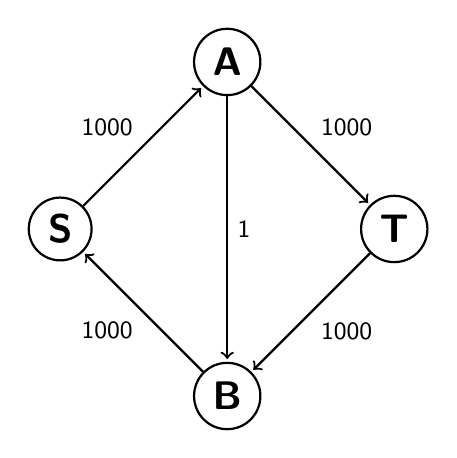
\begin{tikzpicture}[->,shorten >=1pt,auto,node distance=3cm,
                    thick,main node/.style={circle,draw,font=\sffamily\Large\bfseries}]

  \node[main node] (1) {A};
  \node[main node] (2) [below left of=1] {S};
  \node[main node] (3) [below right of=2] {B};
  \node[main node] (4) [below right of=1] {T};

  \path[every node/.style={font=\sffamily\small}]
    (1) edge node [bend left] {1000} (4)
        edge node {1} (3)
    (2) edge node [bend right] {1000} (1)
    (3) edge node [bend right] {1000} (2)
    (4) edge node [bend left] {1000} (3);
\end{tikzpicture}\par
}
 
\begin{itemize}
\item[{\bf (a)}] Show that, if Ford-Fulkerson algorithm is run on this graph, 
  a careless choice of updates might cause it to take 1000 iterations. 
  Imagine if the capacities were a million instead of 1000!

  For all edges in a path from $s - t$ each iteration of the Ford-Fulkerson 
  algorithm updates the max flow based on the edge that has the minimum 
  value of $capacity(edge) - current\_flow(edge)$.  In the case of this graph, if we 
  first update the path S,A,B,T, and then update the path S,B,A,T, then the
  max flow will only increase by one each time. If we continue to alternate between
  these two paths then the maximum flow will only be found after 1000 iterations.
  That is because the max flow
  will increase by one as the path $A-B$ is traveled forward, and then increased
  by one on the next iteration as the path $B- A$ is traveled instead.

   We will now find a strategy for choosing paths under which the algorithm 
   is guaranteed to terminate in a reasonable number of iterations.
   Consider an arbitrary directed network ($G = (V,E),s,t,{c_e}$) in which we 
   want to find the maximum flow. Assume for simplicity that all edge 
   capacities are at least 1, and define the capacity of an $s - t$ path to 
   be the smallest capacity of its constituent edges. 
   The fattest path from $s$ to $t$ is the path with the most capacity.

 \item[{\bf (b)}] Show that the fattest $s - t$ path in a graph can be 
   computed by a variant of Dijkstra's algorithm.

 Since $s$ is the starting vertex, Dijkstra's algorithm usually assigns the 
 distances from all edges away from $s$ to infinity and the distance to $s$ to
 be zero. This is so that the shortest path can be found from $s$ to all other
 vertices. A useful variation would be to preprocess all vertices, not $s$, marking 
 their distances $0$. The distance definition in this case is actually a
 representation of the fat-ness of the path to that node. 

 Instead of updating each node with minimum distance to that node, as with the
 usual Dijkstra implementation, update each vertex with the maximum minimum capacity to that 
 vertex. In practice, all nodes in the graph will start at zero and then increase
 based on the maximum capacity to them. This will continue until all paths to $t$
 have been updated. The vertex $t$ will contain the information about the 
 maximum capacity up to $t$. Note, the maximum capacity path to $t$ must contain
 edges whose maximum capacities are at least the final maximum capacity. 
 To reconstruct the path $s - t$ with maximum 
 capacity, simply traceback the path from $t$ to $s$ based on the largest 
 capacity at each step (breaking ties arbitrarily). This maximum capacity
 path from $s - t$ is the fattest path, by definition. 

\item[{\bf (c)}] Show that the maximum flow in $G$ is the sum of the individual
  flows along at most $E$ paths from $s - t$.
  
  
  

\item[{\bf (d)}] Now show that if we always increase flow along the 
  fattest path in the residual graph, then the Ford-Fulkerson algorithm will 
  terminate in at most $O(|E|\log F)$ iterations, where $F$ is the size of the 
  maximum flow. (Hint: It might help to recall the proof for the greedy set 
  cover algorithm in Section 5.4)

\end{itemize}

In fact, an even simpler rule - finding a path in the residual graph using 
breadth-first search - guarantees that at most $O(|V||E|)$ iterations will 
be needed.

\label{pg:end-of-p3}

% Make sure that the solution here does not exceed one page here. If
% it does, use the extra space for this problem at the end.  
%
% Comment out the next line if you are NOT using the extra space
% \paragraph{} \emph{Continued on Page \pageref{pg:p3-continuation}}

\newpage

\section*{4.  (15 pts.) Evacuation Emergency}

\begin{itemize}
  \item There are $|V|$ rooms in the building.
  \item The start room $s$. You wish to know the maximum number of people 
    who can leave this room safely in $T$ seconds.
  \item Rooms are connected to each other by one-way hallways. You have $|E|$
    hallways total, with the hallway $(u,v,c_{uv},t_{uv})$ connecting room $u$
    to room $v$ having a maximum capacity of $c_{uv}$ people and transit 
    time $t_{uv}$ seconds. At every second, this hallway can only send out 
    $c_{uv}$ from room $u$, and it takes those people $t_{uv}$ seconds to make 
    it to room $v$. Notice, this means that a hallway may contain up to 
    $c_{uv} \times t_{uv}$ people in it at any moment in time. 
    You may also assume the rooms can hold an arbitrarily large number of 
    people who can wait in the room without using a hallway.
\end{itemize}

You may assume that the capacities, transit times, and $T$ are all integers. 
You want to know the maximum value of $N$ such that if $N$ people begin at $s$ 
at time $0$, they can all reach $t$ in at most time $T$ using the hallways. 
Given the rooms $V$ , hallways $E$ , and start and end rooms, show how maximum 
flow in a modified graph can be used to solve this problem
Hint: Consider creating $T$ copies of each room.

Construct a graph $G$ with $T*|V|$ vertices that represent each of the rooms.
The reason for making $T$ 
copies of each of the rooms and hallways is so that each representation of the $|V|$ 
rooms is that room at some time $t, 0\leq t \leq T$. There are also $T$ copies of 
both $s$ and $t$. For some room  $v$, the state of the room at time $t$ is 
represented by the vertex $v_t$ in the graph.

The transit time for some maximum group size $c_{uv}$ from room $u$ to
room $v$, $t_{uv}$ is positive. This means that there is a constraint on the 
capacities of all edges that connect rooms at the same time label, or with a past
time label. For example, two rooms $u_a$ and $v_b$ can only have a nonnegative 
person transfer capacity if $b-a \leq t_{uv}$. This constraint ensures that people
will only move forward in time, as defined by transit times $t_{uv}$. 

The remaining constraint is that there can only be $c_{uv}\times t_{uv}$ in a given
hallway between $u$, and $v$. The careful constraint on person transfer capacities 
based on transit time also contrains the number of people that will be in a hallway
at any one time to $c_{uv}\times t_{uv}$. To illustrate this fact, imagine that 
there are two rooms $u$ and $v$ that have a transit time $t_{uv}=a$ and capacity 
$c_{uv}=b$, we know that the maximum capacity of the hallway is $a\times b$.
At time $t=0$ allow $b$ people to enter the hallway from $u_0$ only to emerge
at $v_a$. Do this again at time $t=1$, $u_1\rightarrow v_{a+1}$. 
Continue this process through $u_{a-1}$. At time state $u_a$, when we release
$b$ more people to travel along hallway $u - v$, the first group of $b$ people has
arrived at $v_a$, leaving only $a\times b$ people in the hallway. 
This shows that there are at most $a\times b$ people in the hallway at any time
with this capacity contraint.



\label{pg:end-of-p4}

% Make sure that the solution here does not exceed one page here. If
% it does, use the extra space for this problem at the end.  
%
% Comment out the next line if you are NOT using the extra space
\paragraph{} \emph{Continued on Page \pageref{pg:p4-continuation}}

\newpage

\section*{5. (20 pts.) Directed Decomposition}

Consider a directed acylcic graph. We define a path to be starting at any 
node $u$ and traversing $0$ or more edges of the DAG and ending at an arbitrary 
node $v$ (if we travel through $0$ edges, we have $u = v$). A path $P$ 
consists of the set of nodes that we touch between $u$ and $v$ (inclusive). 
We wish to find the minimum number of paths such that every vertex is in 
exactly one of these paths. Show how maximum matching in an appropriate 
bipartite graph can be used to solve the problem of determining the 
minimum number of paths needed to cover a DAG.

In order to apply bipartite matching to the DAG we must first construct a 
bipartite graph that represents the DAG appropriately. Let $U$ and $V$ 
be the two sets of vertices of the bipartite graph that are initially empty, but will contain
all of the vertices of the given DAG. Start a BFS at the root of the DAG, 
and let the root vertex be called $v_0$. Add $v_0$ to $U$. Let a vertex $i$
connected to $v_0$ by an edge be called $v_{1_i}$. Add each of these vertices 
to $V$. Continue the BFS search and at each iteration (level in the DAG)
add all even level vertices $v_{even}$ to $U$ and all odd level vertices $v_{odd}$ to $V$.
This construction of $U$ and $V$ does not gurantee a bipartite graph, however. 
In order to ensure a bipartite graph, the BFS search must additionally 
only account for vertices connected by tree edges. All cross and forward 
edges should also be removed in the bipartite representation. 
This will ensure that no 
vertex in $V$ (or $U$) is connected by an edge to another vertex in $V$ (or $U$).

After the bipartite graph is constructed we can create arbitrary sink and source 
nodes, $s$ and $t$. Create edges from $s$ to all vertices in $U$, and create 
edges from all vertices in $V$ to $t$. This generates   


\label{pg:end-of-p5}


% Make sure that the solution here does not exceed one page here. If
% it does, use the extra space for this problem at the end.  
%
% Comment out the next line if you are NOT using the extra space
% \paragraph{} \emph{Continued on Page \pageref{pg:p5-continuation}}

\newpage

% 
%  \section*{6. (10 pts.) Problem 7.21, Flows through cuts}
% 
% \label{pg:end-of-p6}
% 
% % Make sure that the solution here does not exceed one page here. If
% % it does, use the extra space for this problem at the end.  
% %
% % Comment out the next line if you are NOT using the extra space
% %\paragraph{} \emph{Continued on Page \pageref{pg:p6-continuation}}
% 
% \newpage
% 

% Comment out the "extra spaces" completely for the problems for you
% don't neethem
 
 \section*{Extra space for Problem 1}
 \emph{Continued from Page \pageref{pg:end-of-p1}}
 \label{pg:p1-continuation}

Joey will try to maximize his defensive strategy by choosing a strategy that
will be optimal against the optimal startegy that Tony will choose.
$$\mbox{Joey choose:} (x_1,x_2)\mbox{ that maximizes \emph{min}:}\{2x_1-x_2,-2x_2,-3x_1+x_2\}$$
$$z=\emph{min}\{2x_1-x_2,-2x_2,-3x_1+x_2\}$$
\begin{equation*}
  \begin{aligned}
    \mbox{max } z &\\
    2x_1-x_2+z&\leq 0\\
    -2x_2+z&\leq 0\\
    -3x_1+x_2+z&\leq 0\\
    x_1+x_2 &= 1\\
    x_1,x_2&\geq 0\\
  \end{aligned}
\end{equation*}
 
Alternatively, Tony will try to maximize his defensive strategy by choosing a strategy that
will be optimal against the optimal startegy that Joey will choose.
$$\mbox{Tony choose:} (y_1,y_2,y_3)\mbox{ that minimizes \emph{max}:}\{2y_1-3y_3,-y_1-2y_2+y_3\}$$
$$w=\emph{max}\{2y_1-3y_3,-y_1-2y_2+y_3\}$$
\begin{equation*}
  \begin{aligned}
    \mbox{min } w &\\
    -2y_1+3y_3+w&\geq 0\\
    y_1+2y_2-y_3+w&\geq 0\\
    y_1+y_2+y_3 &= 1\\
    y_1,y_2,y_3&\geq 0\\
  \end{aligned}
\end{equation*}

\emph{Solve the LP. Show that the solutions to both are the same and then plug
in the determined X and Y to show the value of the problem}

% \newpage
 %%Comment out the above three lines if you are not using extraspace
 %%for this problem.
 
 
 %\section*{Extra space for Problem 2}
 %\emph{Continued from Page \pageref{pg:end-of-p2}}
 %  
 %\label{pg:p2-continuation}
% %\newpage
% %%Comment out the above three lines if you are not using extra space
% %%fo: r this problem.
% 
% \: section*{Extra space for Problem 3}
% \: emph{Continued from Page \pageref{pg:end-of-p3}}
% 
% \label{pg:p3-continuation}
%
\newpage
%Comment out the above three lines if you are not using extra space
%for this problem.
 
\section*{Extra space for Problem 4}
\emph{Continued from Page \pageref{pg:end-of-p4}}

Here is an example graph where there is a start room $s$, one intermediate room
$u$, an end room $t$, and an exit time of $T=3$. In this graph there are only 
unit transit times. By inspection, this example only has one possible path to
reach the exit in time and the number of people that can exit is defined by 
$\mbox{min}\{c_{su},c_{ut}\}$

{
\centering
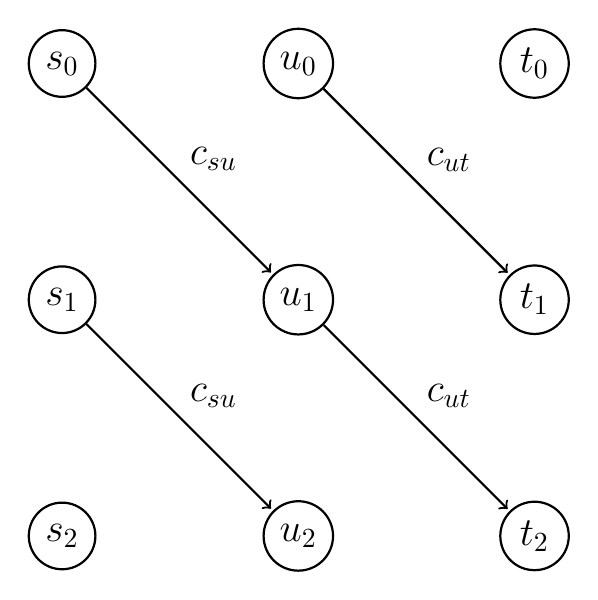
\begin{tikzpicture}[->,shorten >=1pt,auto,node distance=3cm,
                    thick,main node/.style={circle,draw,font=\sffamily\Large\bfseries}]

  \node[main node] (1) {$s_0$};
  \node[main node] (2) [below of=1] {$s_1$};
  \node[main node] (3) [below of=2] {$s_2$};
  \node[main node] (4) [right  of=1] {$u_0$};
  \node[main node] (5) [below of=4] {$u_1$};
  \node[main node] (6) [below of=5] {$u_2$};
  \node[main node] (7) [right of=4] {$t_0$};
  \node[main node] (8) [below of=7] {$t_1$};
  \node[main node] (9) [below of=8] {$t_2$}; 
  \path[every node/.style={font=\sffamily\Large}]
    (1) edge node {$c_{su}$} (5)
        %edge node {$c_{su}$} (6)
    (2) edge node {$c_{su}$} (6)
    (4) edge node {$c_{ut}$} (8)
        %edge node {$c_{ut}$} (9)
    (5) edge node {$c_{ut}$} (9);
\end{tikzpicture}\par
}

To find the maximum flow of people through the rooms at time T, you can simply
run the max-flow algorithm on the constructed graph with $T*|V|$ vertices, and
capacities defined by time and space contraints. 

Proof: The capacities on the graph constrain the number of people that are allowed
to pass and when, as defined by space and time constraints. The defined capacities 
do not allow people to
pass through a hallway unless they have sufficient time and space to do so. Since
the capacities take into account the time and space constraints of movement, the
maximum flow of people through the school is simply defined by the max-flow 
through the graph. 

\label{pg:p4-continuation}
\newpage
 %%Comment out the above three lines if you are not using extra space
 %%for this problem.
 
 
% \section*{Extra space for Problem 5}
% \emph{Continued from Page \pageref{pg:end-of-p5}}
% 
% \label{pg:p5-continuation}
% \newpage
 %%Comment out the above three lines if you are not using extra space
 %%for this problem.
%
% \section*{Extra space for Problem 6}
%% \emph{Continued from Page \pageref{pg:end-of-p6}}
%%%% 
% 
% %Insert solution here
%%%% 
% 
% \label{pg:p6-continuation}
% \newpage
%%Comment out the above three lines if you are not using extra space
%%for this problem.



\end{document}
